\documentclass[acmsmall,review,anonymous,screen]{acmart}
\usepackage{booktabs}
\usepackage{multirow}
\usepackage{makecell}
\usepackage{tikz}
\usetikzlibrary{arrows.meta,positioning,fit,calc,backgrounds}
\usepackage{algorithm}
\usepackage[noend]{algpseudocode}

\setcopyright{none}
\acmJournal{TECS}
\acmYear{2026}

\newcommand{\pol}[1]{\texttt{#1}}
\newcommand{\Wu}{$\mathcal{W}_u$}
\newcommand{\Wl}{$\mathcal{W}$}

\begin{document}

\title{Deadline Miss Early Detection for DAG Tasks with Cross-Frame State and Window Guarantees Under Intervention}

\author{Anonymous Author(s)}
\affiliation{\institution{Submission under double-blind review}\country{}}

\begin{abstract}
Autonomous systems process sensor data through directed acyclic graphs (DAGs) of tasks that must meet end-to-end deadlines. If a
deadline miss is predicted early, the system can reduce the work of the current frame or switch to a lighter fallback before the miss
occurs. Conventional early-detection methods compute, at each node, the probability that the remaining nodes finish in time, from
per-node execution-time distributions. This paper shows that any such score that depends only on the elapsed time of the current
frame is identical for all frames at release, when degradation is cheapest, and that on embedded boards the missing information is
contention that persists across frames. This paper proposes a method that adds a cross-frame contention state to probabilistic laxity
and places a score-agnostic guarantee layer on top of it. The guarantee layer bounds the long-run rate of deadline misses that receive
no warning, bounds the number of such misses in every window of $K$ frames with the fewest possible forced warnings, and, with a
lighter fallback mode, bounds all late frames in every window in an exact form that states how the bound degrades when the fallback
itself is late. All bounds remain valid when the system acts on the warnings. The paper also identifies intervention latch-up, a
failure in which a monitor that acts on its warnings loses the evidence it needs to stop, and fixes it. Pre-registered experiments on
two embedded boards with a live ROS~2 LiDAR pipeline, an independent exhaustive check of the theorems, and a replay of 48,000 logged
release decisions confirm the theorems exactly; a pre-registered replication on seven new seeds and a fallback stress test confirm
them again, with no level-2 frame late in 2{,}544. The experiments also delimit the claims. The predictor does not rank frames better
than logistic regression, the replication did not confirm that the monitor reduces misses at light load, and on the Raspberry Pi~5 at a 6\,ms deadline the fallback itself is late, so only the exact form of the
window bound holds there.
\end{abstract}

\begin{CCSXML}
<ccs2012><concept><concept_id>10010520.10010570</concept_id><concept_desc>Computer systems organization~Real-time systems</concept_desc>
<concept_significance>500</concept_significance></concept></ccs2012>
\end{CCSXML}
\ccsdesc[500]{Computer systems organization~Real-time systems}
\keywords{Deadline miss early detection, DAG, probabilistic execution time, weakly-hard constraint, adaptive conformal inference,
ROS~2, runtime monitoring}

\maketitle

% =====================================================================================================================================
\section{Introduction}\label{sec:intro}

Autonomous vehicles and mobile robots process sensor data through chains of perception, localization and planning tasks, and each
chain must deliver its result within an end-to-end deadline. Platforms such as Autoware~\cite{kato2018autoware} organize this
processing as directed acyclic graphs (DAGs) of nodes in the Robot Operating System 2 (ROS~2)~\cite{macenski2022ros2}. On the
embedded multicore boards used in such systems, worst-case execution time (WCET) analysis of a full ROS~2 graph is rarely available,
other software shares the cores and the memory system, and deadline misses occur in practice. What the system can do is react early:
it can process fewer points, skip a refinement step, or switch to a cheaper estimator, provided that it learns in time that the current
frame is at risk.

Early detection of deadline misses for DAG tasks has been studied in a line of work by Azumi and colleagues. Yano and
Azumi~\cite{yano2023access} assigned time constraints to each job from the end-to-end deadline and WCETs and checked the start time of
each job against them. Toba and Azumi~\cite{toba2024} replaced WCETs by probabilistic execution times and introduced probabilistic
laxity (plaxity). Toba, Baruah and Azumi~\cite{toba2026} further introduced workload-dependent probability thresholds, increasing
the threshold as the remaining workload shrinks. That work establishes the probabilistic-laxity baseline used here. The present paper
addresses a different question: how to use information that persists across frames and how to preserve a monitor's guarantees after
its warnings trigger actions.

This paper takes up that direction and identifies two limitations that appear once the detector is used to act. First, plaxity is
\emph{blind at release}. The plaxity of a frame depends only on that frame's elapsed time, which is zero for every frame at release,
so every frame receives the same score at the moment when degrading the whole frame is cheapest. This holds for any execution-time
distribution and any threshold (Theorem~\ref{thm:blind}). On embedded boards, slow frames are caused mainly by contention from other
software. Such contention slows every node of a frame together and persists across frames, so it is visible before the frame starts,
but only to a method that carries state across frames. Second, \emph{a detector is not designed to be acted upon}. When the system
degrades the frames that the detector warns about, three requirements appear:
\begin{itemize}
\item the detector's data become shaped by its own actions, and any guarantee it offers must survive this;
\item a downstream controller needs a bound on every short window of frames, not only on a long-run average;
\item a warned frame is useful only if the degraded mode actually finishes in time.
\end{itemize}

To address these limitations, this paper proposes a deadline miss early detection method with two layers. The \emph{prediction layer}
keeps the plaxity of Toba et al.~\cite{toba2024,toba2026} and conditions it on a cross-frame contention state, updated from completed
frames and from the nodes of the current frame. The \emph{guarantee layer} is independent of the prediction layer. It consists of an
adaptive threshold that bounds the long-run rate of unwarned deadline misses, and of a counting rule that bounds unwarned misses, or,
with a lighter fallback mode, all late frames, in every window of $K$ frames. The prediction layer only decides how many false alarms
are needed to meet the guarantees; it never decides whether they hold.

The main contributions of this paper are summarized as follows:
\begin{itemize}
\item Establishing the release-time blindness of elapsed-time-only early-detection scores, including plaxity under arbitrary
execution-time distributions and thresholds, and introducing cross-frame contention state to provide information before a frame
begins (Sections~\ref{sec:blind} and~\ref{sec:kp}).
\item Developing a score-agnostic guarantee layer comprising a long-run bound on unwarned misses, a lag-correct $(m,K)$ window bound
with a minimality result and a bound on the warnings it forces, and an all-late-frame bound that explicitly accounts for late level-2
fallback frames (Sections~\ref{sec:aci}--\ref{sec:all}).
\item Identifying intervention latch-up and introducing a mode-aware state update, while establishing the necessity of the monitor's
components and positioning the combined contract against bounded-miss scheduling, $(m,k)$-firm scheduling, adaptive conformal
inference and weakly-hard monitoring (Sections~\ref{sec:latch} and~\ref{sec:position}).
\item Evaluating the method through pre-registered experiments on two embedded boards with a live ROS~2 pipeline, independent
exhaustive checks of the theorems and an implementation-conformance replay, while reporting failed tests and unsupported assumptions
alongside successful results (Section~\ref{sec:eval}).
\end{itemize}

\paragraph{Scope of the claims} The paper does not claim a better predictor: logistic regression on the same features ranks frames as
well as the proposed predictor (Section~\ref{sec:eval-open}). The paper does not claim that the fallback is always on time: on one of
the two boards and one of its deadlines it is not, and only the exact form of the window bound holds there (Section~\ref{sec:eval-fb}).
Table~\ref{tab:claims} at the end of Section~\ref{sec:eval} lists every claim with its premise and its status.

The remainder of this paper is structured as follows. Section~\ref{sec:model} outlines the system model. Section~\ref{sec:problem}
specifies the problem model, including the requirements on a monitor that is acted upon and the position of this work against existing
mechanisms. Section~\ref{sec:method} details the proposed method. Section~\ref{sec:eval} presents the evaluation results.
Section~\ref{sec:related} reviews related work. Section~\ref{sec:concl} concludes with future research directions.

% =====================================================================================================================================
\section{System Model}\label{sec:model}

This section presents the system model used in this paper, including the DAG model, the execution-time and contention model, and the
actions available to the monitor. The notations are summarized in Table~\ref{tab:notation}.

\begin{table}[t]
\caption{Notations}
\label{tab:notation}
\footnotesize
\begin{tabular}{@{}ll@{}}
\toprule
Symbol & Description \\
\midrule
$G=(V,E)$ & DAG with nodes $V=\{\tau_1,\dots,\tau_n\}$ and edges $E$ \\
$t$ & Frame (job of the DAG) index; frame $t$ is released at time $tP$ \\
$P$, $D$ & Period and relative end-to-end deadline \\
$C_t$ & End-to-end response time of frame $t$; frame $t$ is \emph{late} if $C_t>D$ or it never finishes \\
$k$, $E_{t,k}$ & Checkpoint index ($k=0$: release) and elapsed time of frame $t$ at checkpoint $k$ \\
$\pi_k(e)$ & Plaxity: probability that the remaining nodes finish within $D-e$ \\
$z_t$ & Cross-frame contention state (log scale) \\
$s_{t,k}$ & Miss score of frame $t$ at checkpoint $k$ \\
$\theta_t$, $\alpha$, $\gamma$ & Adaptive alarm threshold, target rate, step \\
$L$ & Feedback lag: the outcome of frame $t$ is known by the release of frame $t+L$ \\
$(m,K)$ & Window budget: at most $m$ counted frames in any $K$ consecutive frames \\
$e_t$ & 1 if frame $t$ is an unwarned deadline miss, else 0 \\
$c_t$, $c^u_t$ & Window counters of rules \Wl{} and \Wu{} at the release of frame $t$ \\
\bottomrule
\end{tabular}
\end{table}

\subsection{DAG-based Workload Model}

The application is represented as a DAG $G=(V,E)$ whose nodes are tasks and whose edges are data flow between tasks. A single entry
node is triggered by a timer with period $P$; the other nodes are triggered by the arrival of data from their predecessors, as in the
event-driven nodes of~\cite{yano2023access,toba2026}. Each release of the entry node starts a \emph{frame}, which ends when the exit node
finishes. A deadline $D\le P$ is assigned to the exit node.

The main workload of this paper is a LiDAR perception DAG on nuScenes scans~\cite{caesar2020nuscenes}, illustrated in
Fig.~\ref{fig:sys}. N1 loads and crops the scan; N2 voxelizes it; N3 (ground and obstacle grid) and N4 (height map) run in parallel;
N5 fuses their outputs into free-space sectors; $P=100$\,ms. A second DAG performs visual odometry on EuRoC
frames~\cite{burri2016euroc} with $P=200$\,ms. Both DAGs run as five \texttt{rclcpp} nodes in one ROS~2 Jazzy process with a
multi-threaded executor.

\begin{figure}[t]
\centering
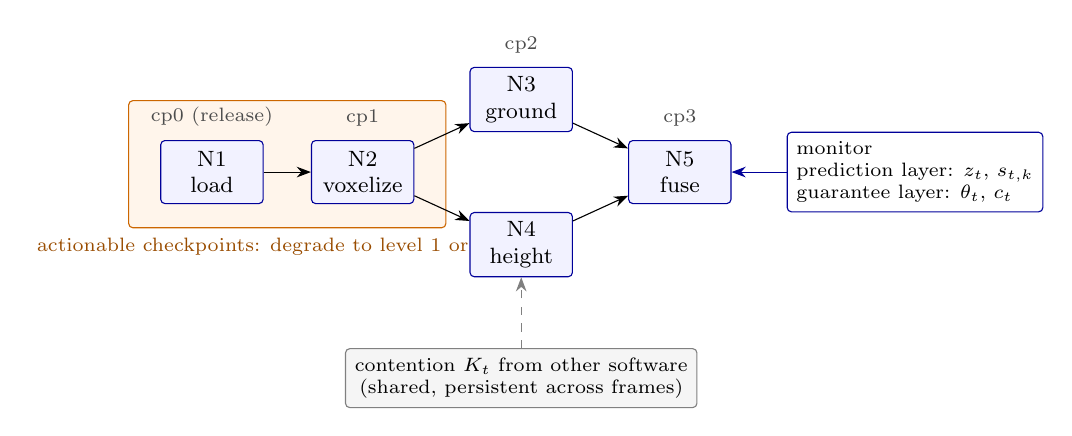
\begin{tikzpicture}[font=\footnotesize, node distance=6mm,
  nd/.style={draw=blue!60!black, fill=blue!5, rounded corners=1.5pt, minimum width=13mm, minimum height=8mm, align=center},
  cp/.style={font=\scriptsize, text=black!70}]
\node[nd] (n1) {N1\\load};
\node[nd, right=of n1] (n2) {N2\\voxelize};
\node[nd, above right=1mm and 7mm of n2] (n3) {N3\\ground};
\node[nd, below right=1mm and 7mm of n2] (n4) {N4\\height};
\node[nd, below right=1mm and 7mm of n3] (n5) {N5\\fuse};
\foreach \a/\b in {n1/n2,n2/n3,n2/n4,n3/n5,n4/n5} \draw[-{Stealth[length=1.8mm]}] (\a) -- (\b);
\node[cp, above=0.5mm of n1] {cp0 (release)};
\node[cp, above=0.5mm of n2] {cp1};
\node[cp, above=0.5mm of n3] {cp2};
\node[cp, above=0.5mm of n5] {cp3};
\begin{scope}[on background layer]
\node[draw=orange!80!black, fill=orange!8, rounded corners=1.5pt, fit=(n1)(n2), inner sep=4mm, yshift=1mm,
      label={[font=\scriptsize, text=orange!60!black]below:actionable checkpoints: degrade to level 1 or level 2}] {};
\end{scope}
\node[draw=black!50, fill=black!4, rounded corners=1.5pt, align=center, below=9mm of n4, font=\scriptsize] (cont)
      {contention $K_t$ from other software\\(shared, persistent across frames)};
\node[draw=blue!60!black, rounded corners=1.5pt, align=left, right=7mm of n5, font=\scriptsize] (mon)
      {monitor\\prediction layer: $z_t$, $s_{t,k}$\\guarantee layer: $\theta_t$, $c_t$};
\draw[-{Stealth[length=1.8mm]}, dashed, black!50] (cont) -- (n4);
\draw[-{Stealth[length=1.8mm]}, blue!60!black] (mon) -- (n5);
\end{tikzpicture}
\caption{The LiDAR DAG, its checkpoints and the monitor. Only alarms at cp0 and cp1 can still save the frame by degrading it.}
\label{fig:sys}
\end{figure}

\subsection{Execution Time and Contention}

The execution time of each node is a random variable, as in~\cite{toba2024,toba2026}. Unlike the independence assumption used there,
this paper models the dominant source of dependence explicitly. Other software, here Autoware reference-system
processes~\cite{refsystem} or ordinary applications (a compiler, compressors and a Python workload), runs concurrently and shares the
cores and the memory system. The number of concurrent interferers $I_t\in\{0,1,2,3\}$ switches at random with exponential dwell times.
Calibration data contain $I_t\in\{0,1,2\}$; validation data add $I_t=3$ and, in later experiments, an interferer type never seen in
calibration. Contention slows all nodes of a frame together and persists across frames, so execution times are dependent within and
across frames.

\subsection{Monitor, Actions and Fallback Modes}

A monitor is evaluated at four checkpoints (Fig.~\ref{fig:sys}): the release of the frame (cp0), the start of N2 (cp1), the start of the
fork (cp2) and the start of N5 (cp3). An alarm at cp0 or cp1 is \emph{actionable}, because the frame can still be degraded. Two
degradation levels exist. \emph{Level~1} keeps every second point of the scan and \emph{level~2} keeps every eighth point; both shorten
N2--N5. A frame is \emph{warned} if it was degraded at release or raised an alarm at an actionable checkpoint. An \emph{unwarned
deadline miss} is a late frame that was not warned. The outcome of frame $t$ (late or not) becomes known to the monitor when the frame
finishes; a frame that has not finished is \emph{running}. The feedback lag $L$ bounds how many releases may pass before an outcome
is known.

% =====================================================================================================================================
\section{Problem Model}\label{sec:problem}

This section specifies the problem. Section~\ref{sec:blind} shows why per-frame early detection cannot act at release.
Section~\ref{sec:req} states the requirements on a monitor whose warnings are acted upon. Section~\ref{sec:position} delimits what
existing mechanisms provide and what they do not.

\subsection{Release-Time Blindness of Per-Frame Early Detection}\label{sec:blind}

The plaxity of Toba et al.~\cite{toba2024,toba2026} at checkpoint $k$ and elapsed time $e$ is $\pi_k(e)=\Pr[R_k\le D-e]$, where the
remaining time $R_k$ is the convolution of the execution-time distributions of the unfinished nodes. An alarm is raised when
$\pi_k(e)$ falls below a threshold $th_k$, which rises towards the exit node~\cite{toba2026}. The function $\pi_k$ is fixed after
calibration, and its only run-time argument is the elapsed time of the current frame. Let $\mathcal I_{t,k}$ denote the information
available at checkpoint $k$ of frame $t$, and $Y_t=\mathbf 1[C_t>D]$.

\begin{theorem}[Release-time blindness]\label{thm:blind}
Let $s_{t,k}=g_k(E_{t,k})$ for fixed functions $g_k$; this includes plaxity with any distributions, fork rule and thresholds. Then
(i) at release, $s_{t,0}=g_0(0)$ for every frame, its AUROC for $Y_t$ is exactly $1/2$, and every threshold raises an alarm on all frames
or on none; (ii) if $g_k$ is monotone, the ROC curve of $s_{t,k}$ is dominated by that of $E_{t,k}$ itself.
\end{theorem}
\begin{proof}
(i) $E_{t,0}=0$ for every $t$, so the score is constant; every pair of a late and an on-time frame is tied, and a threshold on a
constant is all-or-nothing. (ii) The ROC curve is invariant under strictly monotone transformations of the score; a non-strictly
monotone transformation only merges scores into ties, which replaces parts of the curve by chords of it.
\end{proof}

\begin{proposition}[Information limit]\label{prop:limit}
Among $\mathcal I_{t,k}$-measurable scores, $p^\star_{t,k}=\Pr[Y_t=1\mid\mathcal I_{t,k}]$ has the highest ROC curve, and enlarging
$\mathcal I_{t,k}$ cannot lower it. If $\log C_t=S_t+\varepsilon_t$ with a state $S_t$ known at release and independent Gaussian noise
$\varepsilon_t$, the best release-time AUROC depends only on $R^2=\mathrm{Var}(S_t)/\mathrm{Var}(\log C_t)$ and on the miss rate.
\end{proposition}
\begin{proof}
By the Neyman--Pearson lemma, the most powerful test at every false-positive rate thresholds the likelihood ratio, which is a monotone
function of $p^\star_{t,k}$; an $\mathcal I'$-measurable score is also $\mathcal I$-measurable for $\mathcal I'\subseteq\mathcal I$. In the
Gaussian case $p^\star_{t,0}$ is monotone in $S_t$.
\end{proof}

Theorem~\ref{thm:blind} states that no choice of distributions can make per-frame early detection act at release; better detection at
release must come from information available before the frame starts. Proposition~\ref{prop:limit} states how much any method can gain
from such information.

\subsection{Requirements for a Monitor That Is Acted Upon}\label{sec:req}

On a platform without WCET analysis, a monitor whose warnings trigger degradation should satisfy six requirements.
\begin{description}
\item[R1] It warns at release, when degradation is cheapest.
\item[R2] It gives a hard $(m,K)$ bound in every window of $K$ frames, not only a long-run rate.
\item[R3] R2 still holds when outcomes become known only after a lag $L\ge1$, the normal case in a pipelined system.
\item[R4] Its guarantees remain valid when its own actions shape the data from which it learns.
\item[R5] It bounds \emph{all} late frames, not only unwarned ones, and states how the bound degrades when the fallback is late.
\item[R6] A learned predictor decides only the false-alarm price, never whether a guarantee holds.
\end{description}

\subsection{What Existing Mechanisms Provide, and What They Do Not}\label{sec:position}

Each ingredient of the proposed method exists in some form. This subsection states precisely what each line of work provides on its
own, what the proposed method takes from it, and what it adds. Table~\ref{tab:compare} summarizes the comparison in the style
of~\cite{toba2026}.

\begin{table}[t]
\caption{Comparison of the proposed method with related work. \checkmark: provided; $\circ$: provided under the stated extra
assumption; --: not provided or out of scope.}
\label{tab:compare}
\footnotesize
\begin{tabular}{@{}lccccccc@{}}
\toprule
Work & DED$^a$ & R1 & R2 & R3 & R4 & R5 & R6 \\
\midrule
Yano and Azumi, IEEE Access 2023~\cite{yano2023access} & \checkmark & -- & -- & -- & -- & -- & -- \\
Toba and Azumi, ECRTS 2024~\cite{toba2024}; Toba et al., TECS 2026~\cite{toba2026} & \checkmark & -- & -- & -- & -- & -- & -- \\
Bernat and Cayssials, RTSS 2001 (Bi-Modal Scheduler)~\cite{bernat2001bms} & -- & -- & $\circ^b$ & $\circ^c$ & -- & $\circ^b$ & -- \\
Hamdaoui and Ramanathan, TC 1995 ($(m,k)$-firm)~\cite{hamdaoui1995} & -- & -- & $\circ^b$ & $\circ^c$ & -- & -- & -- \\
Gibbs and Cand\`es, NeurIPS 2021 (ACI)~\cite{gibbs2021} & -- & -- & -- & \checkmark & $\circ^d$ & -- & \checkmark \\
Peeck et al., DATE 2021~\cite{peeck2021} & \checkmark$^e$ & -- & $\circ^f$ & -- & -- & $\circ^g$ & -- \\
Wu et al., RV 2020~\cite{wu2020rv} & -- & -- & $\circ^h$ & -- & -- & -- & -- \\
Jiang et al., RTSS 2020 (Pythia-MCS)~\cite{jiang2020pythia} & \checkmark & $\circ^i$ & -- & -- & -- & -- & -- \\
Proposed method & \checkmark & \checkmark & \checkmark & \checkmark & \checkmark & \checkmark$^j$ & \checkmark \\
\bottomrule
\end{tabular}

\vspace{2pt}
\parbox{\textwidth}{\scriptsize
$^a$ DED: deadline miss early detection at run time.
$^b$ Given a schedulability (WCET) analysis that guarantees the switched-to mode.
$^c$ Outcomes known at each job's deadline.
$^d$ Long-run rate only; the bound is sequence-wise.
$^e$ Detection after a segment budget is overrun.
$^f$ $(m,k)$ checked on measured traces when the budgets are set; not enforced online.
$^g$ Fallback to a safety layer whose timing is assumed.
$^h$ The system is verified \emph{if} the environment satisfies the constraints; otherwise it switches to a safe mode.
$^i$ Before the overrun, from I/O behaviour, to trigger a mixed-criticality mode switch.
$^j$ Exact form without assumption; plain form only when the fallback is on time.}
\end{table}

\paragraph{Bounded-miss scheduling} The Bi-Modal Scheduler of Bernat and Cayssials~\cite{bernat2001bms} runs jobs in a best-effort mode
and switches to a guaranteed panic mode when one more miss would violate the weakly-hard constraint~\cite{bernat2001weakly}.
$(m,k)$-firm scheduling~\cite{hamdaoui1995} raises the priority of a stream as it approaches a violation. Both count misses against a
window, and the counting rules of this paper use the same idea; it is not claimed as new. The guarantee of both rests on a
schedulability analysis that ensures the guaranteed mode, or the prioritized job, meets its deadline. The proposed method differs in
three precise ways. (i) Its window bound on unwarned misses (Theorem~\ref{thm:wu}) uses no timing analysis at all: the rule acts by
warning, which is always possible, instead of by meeting a deadline. (ii) Its counter is correct under a lag $L$; a counter of known
misses only, as at a scheduler's deadline, admits $m+L-1$ (Proposition~\ref{prop:need}). (iii) For all late frames
(Theorem~\ref{thm:all}) it gives an exact form that holds when the fallback is late, so the timing assumption that bounded-miss
scheduling makes implicitly is separated and can be measured. In the special case $L=1$, a predictor that never warns, and a fallback
that is never late, rule \Wl{} switches on exactly the condition described for the panic mode in~\cite{bernat2001bms}.

\paragraph{Adaptive conformal inference} The long-run bound of Section~\ref{sec:aci} is the one-sided form of the adaptive conformal
inference (ACI) bound of Gibbs and Cand\`es~\cite{gibbs2021}, with a feedback lag; it is not claimed as new mathematics. ACI provides
neither a window bound (Proposition~\ref{prop:need}(2) constructs $\lfloor\theta_1/(\gamma(1-\alpha))\rfloor$ consecutive unwarned misses
under a valid ACI threshold) nor a bound on late frames. The contribution here is its use as one layer of a monitor that is acted upon,
with the observation that the bound remains valid under intervention because it is sequence-wise and is defined only on unwarned
frames.

\paragraph{Weakly-hard monitoring} Peeck, Schlatow and Ernst~\cite{peeck2021} monitor the latency of event chains online with segment
timeouts and fall back to a safety layer; the segment budgets are set on measured traces so that an $(m,k)$ requirement holds on those
traces. Wu et al.~\cite{wu2020rv} verify a system under multiple weakly-hard constraints and switch to a safe mode when the environment
violates them. Both \emph{detect} or \emph{verify} a weakly-hard property; neither \emph{enforces} one online by forcing warnings or
degradation, and detection by timeout happens only after a budget is overrun. The proposed method enforces $(m,K)$ by construction, with
proofs that do not depend on traces.

\paragraph{What the proposed method adds} The contribution is a combination with a specific structure, not any single rule:
\begin{enumerate}
\item a \emph{decomposition of the contract}, in which every guarantee follows from a counter or a threshold update whose proof uses no
timing model and no property of the predictor, so that a learned predictor becomes admissible in a monitor with a hard window contract;
\item \emph{lag-correct counting} of running frames, with a minimality proof;
\item \emph{validity under the monitor's own interventions}, together with the identification and fix of latch-up, the one way in which
intervention does break such a monitor in practice;
\item an \emph{exact, assumption-free window bound on all late frames}, which makes the timing assumption on the fallback explicit,
measurable and budgetable;
\item \emph{release-time warning} from cross-frame state, which per-frame detection cannot provide.
\end{enumerate}
The individual proofs are short, and the following proposition shows that none of the components can be removed.

\begin{proposition}[Each component is necessary]\label{prop:need}
Consider the proposed method with one component removed.
\begin{enumerate}
\item Without cross-frame state, the release decision is the same for every frame (Theorem~\ref{thm:blind}).
\item With the adaptive threshold but no window rule, scores identically 0 and every frame late, the first
$\lfloor\theta_1/(\gamma(1-\alpha))\rfloor$ frames are unwarned misses, so no $(m,K)$ bound holds for $K\le\theta_1/(\gamma(1-\alpha))$
although Theorem~\ref{thm:aci} holds.
\item If the window counter ignores running frames, the worst number of unwarned misses in a window is exactly $\min(m+L-1,K)$.
\item With a window rule on unwarned misses only, every warned frame may be late, so up to $K$ late frames per window are possible
while Theorem~\ref{thm:wu} holds.
\item If the state is updated only from undegraded frames and the monitor degrades every frame after a contention burst, the state never
decreases. With a fixed threshold every later frame is degraded; with the adaptive threshold the latch ends only after the threshold has
risen above the stale score $s$, which takes $(s-\theta_t)/(\gamma\alpha)$ frames and leaves the threshold loosened.
\end{enumerate}
\end{proposition}
\begin{proof}
(1) is Theorem~\ref{thm:blind}. (2) With scores 0, frame $t$ is warned only if $\theta_t<0$, and each fed-back unwarned miss lowers
$\theta$ by $\gamma(1-\alpha)$. (3) At the release of $t$ the frames $t-L+1,\dots,t-1$ may be running and are not counted; with $m-1$
known unwarned misses in the window, $t$ is released unwarned, and an adversary makes the $L-1$ running frames and $t$ late, which gives
$m+L-1$. The upper bound follows from the argument of Theorem~\ref{thm:wu} with $L-1$ uncounted frames. (4) Nothing constrains the
latency of a warned frame. (5) The release prior is a function of undegraded outcomes only; when none arrive it is constant, and a
degraded frame is warned, so $e_t=0$ and $\theta$ rises by $\gamma\alpha$ per frame.
\end{proof}

% =====================================================================================================================================
\section{Proposed Method}\label{sec:method}

This section details the proposed method: the prediction layer (Section~\ref{sec:kp}), the three guarantees
(Sections~\ref{sec:aci}--\ref{sec:all}), the latch-up fix (Section~\ref{sec:latch}) and the complete algorithm
(Section~\ref{sec:alg}).

\subsection{Cross-Frame State: Kalman Plaxity}\label{sec:kp}

The proposed predictor keeps the quantity, checkpoints and convolution of plaxity~\cite{toba2024,toba2026} and adds one state. Let
$z_t$ be a log-scale contention state. At the release of frame $t$, its prior mean is an exponentially weighted average of
$\log(C_j/\bar C)$ over completed frames $j<t$, where $\bar C$ is the median calibration latency. Within the frame, each finished node
$i$ gives a scalar Gaussian observation of $z_t$ from the log of its duration relative to its calibration median. The remaining time is
$e^{z_t}$ times the convolution of the state-normalized node durations, stored as 64 quantiles, and the score is
$s_{t,k}=\Pr[E_{t,k}+R_k>D\mid z_t]$. This predictor is called Kalman plaxity (KP). A variant, KPF, also forms a prior from system
telemetry (CPU and memory counters read by a background sampler) and fuses the two priors online, each weighted by its recent squared
prediction error. The predictor runs inline in the ROS~2 process; its implementation is in C++.

\subsection{Long-Run Guarantee on Unwarned Deadline Misses}\label{sec:aci}

A frame raises an alarm at the first actionable checkpoint at which $s_{t,k}>\theta_t$. When the outcome of frame $t-L$ becomes known,
the threshold is updated as $\theta_{t+1}=\theta_t-\gamma(e_{t-L}-\alpha)$.

\begin{theorem}[Long-run bound]\label{thm:aci}
For any scores in $[0,1]$ and any sequence of response times, including sequences shaped by the monitor's own interventions,
\[\frac1T\sum_{t\le T}e_t\;\le\;\alpha+\frac{\theta_1+(L+1)\gamma}{\gamma T}+\frac LT.\]
\end{theorem}
\begin{proof}
If $\theta_t<0$, every score exceeds $\theta_t$, so $e_t=0$. Hence $\theta$ decreases only after an unwarned miss released at
$\theta\ge0$, and at most $L+1$ decrements of size at most $\gamma$ act after that point, so $\theta_t\ge-(L+1)\gamma$ for all $t$.
Telescoping the update gives $\sum_{u\le T-L}(e_u-\alpha)=(\theta_1-\theta_{T+1})/\gamma\le(\theta_1+(L+1)\gamma)/\gamma$, and the last
$L$ terms add at most $L$.
\end{proof}
The proof uses no exchangeability or stationarity and therefore holds for every individual sequence. Because $e_t$ is defined only on
unwarned frames, which run unmodified, intervention does not change what is measured. The bound is one-sided, which is the
safety-relevant side.

\subsection{Window Guarantee on Unwarned Deadline Misses}\label{sec:wu}

\begin{definition}[Rule \Wu]
Before releasing frame $t$, let $c^u_t=\#\{j\in[t-K+1,t-1]: j$ is a known unwarned miss, or $j$ is unwarned and running$\}$. If
$c^u_t\ge m$, frame $t$ is warned at release (degraded to level~1).
\end{definition}

\begin{theorem}[$(m,K)$ on unwarned misses]\label{thm:wu}
Under rule \Wu, for every predictor, every response-time sequence and every lag, every window of $K$ consecutive frames contains at most
$m$ unwarned deadline misses.
\end{theorem}
\begin{proof}
Suppose a window contains $m+1$ unwarned misses, and let $f$ be the last of them. Frame $f$ was not warned, so $c^u_f<m$. The other $m$
lie in $[f-K+1,f-1]$; at the release of $f$, each is either a known unwarned miss or unwarned and running, so all are counted and
$c^u_f\ge m$, a contradiction.
\end{proof}

\begin{proposition}[Minimality]\label{prop:min}
Any causal policy that guarantees $(m,K)$ on unwarned misses for every response-time sequence must warn every frame that rule \Wu{}
forces.
\end{proposition}
\begin{proof}
If $c^u_t\ge m$, an adversary consistent with all observations makes every counted running frame late and frame $t$ late; unless $t$ is
warned, the window $[t-K+1,t]$ contains $m+1$ unwarned misses.
\end{proof}

Minimality states that no forced warning can be dropped; it does not state how many warnings are forced. The next result bounds that
price in terms of the quantity that the long-run layer already controls, and thereby connects the two layers of the guarantee.

\begin{theorem}[Price of the window rule]\label{thm:cost}
Over any horizon of $T$ frames, let $F$ be the number of frames forced by rule \Wu, $U$ the number of unwarned deadline misses and $N$
the number of unwarned frames. For every predictor, every response-time sequence and every lag~$L$,
\[ mF \;\le\; (K-1)\,U + (L-1)\,N. \]
\end{theorem}
\begin{proof}
Each forced frame $t$ has $c^u_t\ge m$, so $mF\le\sum_t c^u_t$. A frame $j$ contributes to $c^u_t$ only for $t\in[j+1,j+K-1]$, and
only if it is unwarned. If $j$ is an unwarned miss it contributes at most $K-1$ times. If $j$ is unwarned and on time it contributes
only while it is running, which is at most $L-1$ releases by the definition of $L$. Summing over $j$ gives the bound.
\end{proof}

\begin{corollary}[Forced-warning rate]\label{cor:cost}
If the threshold of Section~\ref{sec:aci} runs together with rule \Wu, then for $L=1$
\[ \frac FT\;\le\;\frac{K-1}{m}\left(\alpha+\frac{\theta_1+2\gamma}{\gamma T}+\frac1T\right). \]
\end{corollary}
\begin{proof}
Forced frames are warned, so they only add warnings; the proof of Theorem~\ref{thm:aci} holds unchanged for the combined policy and
bounds $U$. Insert this bound into Theorem~\ref{thm:cost}.
\end{proof}

The two layers therefore support each other: the long-run layer keeps the unwarned-miss rate near $\alpha$, and this caps the fraction of
frames that the window layer can force at $(K-1)\alpha/m$, whatever the predictor and the response times. A budget with
$m/(K-1)$ well above $\alpha$ is cheap; a budget below it can force many warnings, which matches the behaviour observed in
Section~\ref{sec:eval-disc}. For $L=1$ the constant is close to tight: exhaustive enumeration (Section~\ref{sec:eval-verify}) shows that
the largest value of $mF/U$ over all sequences is exactly $K-m$, attained by blocks of $m$ consecutive unwarned misses, each of which
forces the next $K-m$ releases.

\subsection{Window Guarantee on All Late Frames with a Fallback}\label{sec:all}

\begin{definition}[Rule \Wl]
Before releasing frame $t$, let $c_t=\#\{j\in[t-K+1,t-1]: j$ is known late, or $j$ is running and not at level~2$\}$. If $c_t\ge m$,
frame $t$ runs at level~2. Otherwise the prediction layer and the adaptive threshold decide between normal mode and level~1.
\end{definition}

\begin{theorem}[All late frames, exact form]\label{thm:all}
Under rule \Wl, for every response-time sequence and every lag, every window $W$ of $K$ frames satisfies
\[\#\{\text{late frames in }W\}\;\le\;m+\#\{\text{late level-2 frames in }W\}.\]
\end{theorem}
\begin{proof}
It suffices to show that $W$ contains at most $m$ late frames that are not at level~2. If it contained $m+1$, let $f$ be the last; $f$ is
not at level~2, so $c_f<m$, while the other $m$ lie in $[f-K+1,f-1]$ and are each known late or running and not at level~2 at the release
of $f$, so $c_f\ge m$, a contradiction.
\end{proof}

Theorem~\ref{thm:all} makes no assumption on timing. Its only premise is bookkeeping: a frame counts as running until its outcome is
known, which the implementation satisfies (Section~\ref{sec:eval-verify}). Two weaker statements follow, and they require different
evidence.

\begin{corollary}[Budgeted form]\label{cor:r}
If at most $r$ level-2 frames are late in any window of $K$ frames, every window contains at most $m+r$ late frames.
\end{corollary}

\begin{corollary}[Plain form]\label{cor:A}
If level-2 frames are never late (assumption A), every window of $K$ frames contains at most $m$ late frames.
\end{corollary}

Assumption A concerns the platform, the deadline, the contention and the scheduling configuration, not the monitor. A finite measurement
can bound the \emph{rate} of late level-2 frames but cannot establish A deterministically; a deterministic plain form requires a WCET
bound or a reservation for level~2. This paper therefore reports three tiers of results: Theorem~\ref{thm:all} unconditionally,
Corollary~\ref{cor:r} with a measured $r$, and Corollary~\ref{cor:A} only where no level-2 frame was ever late, together with a confidence
bound on the late rate. Minimality carries over as in Proposition~\ref{prop:min}.

If a late frame makes a controller hold its previous command, Corollary~\ref{cor:A} is the precondition of the standard weakly-hard
stability argument~\cite{maggio2020,vreman2021}: for a linear plant with on-time matrix $U$ and hold matrix $H$, the loop is exponentially
stable if $\max_w\lVert\prod_{t\in w}M_t\rVert<1$ over all words $w\in\{U,H\}^K$ with at most $m$ symbols $H$. Under
Corollary~\ref{cor:r}, the same certificate is evaluated with $m+r$.

\subsection{Intervention Latch-Up and the Mode-Aware State Update}\label{sec:latch}

The first closed-loop version of the method updated $z_t$ only from frames that ran in normal mode. Once it degraded a frame, that frame
gave no evidence that contention had ended, so $z_t$ remained high and the next frame was degraded as well. In the logs of the first
closed-loop experiment, the monitor degraded 59--88\% of the frames in quiet periods in which it would have raised an alarm on only
1--3\%. This failure is called \emph{intervention latch-up}: a monitor that acts on its warnings destroys the evidence it needs to stop
warning. It is a concrete timing-monitor instance of the feedback problem studied in conformal prediction under
feedback~\cite{fannjiang2022}. The fix is a \emph{mode-aware} update: frames degraded to level~1 also update $z_t$, normalized by the
typical latency of level~1, which is measured in a short calibration run with random degradation. Level-2 frames do not update the
state; they are triggered only by the window rule, which depends on outcomes and not on the state. The guarantees are unaffected,
because they depend only on unwarned frames (Theorems~\ref{thm:aci} and~\ref{thm:wu}) or on lateness itself (Theorem~\ref{thm:all}).

\subsection{Algorithm}\label{sec:alg}

Algorithm~\ref{alg:mon} shows the per-frame procedure of the proposed method with rule \Wl, as deployed (policy \pol{kpmd}). The
variant with rule \Wu{} (policy \pol{kpmwh}) replaces lines~\ref{ln:c}--\ref{ln:l2} by the counter $c^u_t$ and degrades to level~1.
A burst guard lowers the effective threshold by $\kappa\max(0,b_t-\alpha W_b)$, where $b_t$ is the number of known unwarned misses among
the last $W_b$ frames; it can only add alarms, so no guarantee depends on it. The state is $O(K+W_b)$, and each release costs two window
scans and a few quantile lookups.

\begin{algorithm}[t]
\caption{Proposed method with rule \Wl, per frame $t$}\label{alg:mon}
\small
\begin{algorithmic}[1]
\Require target $\alpha$, step $\gamma$, budget $(m,K)$, burst-guard window $W_b$ and gain $\kappa$
\State $c_t\gets\#\{j\in[t-K+1,t-1]:$ known late, or running and not at level 2$\}$ \label{ln:c}
\If{$c_t\ge m$} mode $\gets$ level 2 \label{ln:l2}
\ElsIf{$s_{t,0}(z_t)>\theta_t-\kappa\max(0,b_t-\alpha W_b)$} mode $\gets$ level 1
\Else{} mode $\gets$ normal \EndIf
\State run N1; update $z_t$ in frame from N1's duration
\If{mode $=$ normal and $s_{t,1}(z_t)>\theta_t-\kappa\max(0,b_t-\alpha W_b)$} degrade the rest of the frame to level 1 \EndIf
\State run N2--N5, updating $z_t$ in frame after each node
\State on completion: if mode $\ne$ level 2, update the cross-frame prior with $\log(C_t/\bar C_{\text{mode}})$ \Comment{mode-aware}
\State on completion: record late or not; $\theta\gets\theta-\gamma(e_t-\alpha)$
\end{algorithmic}
\end{algorithm}

% =====================================================================================================================================
\section{Evaluation}\label{sec:eval}

The performance of the proposed method is evaluated through experiments on two embedded boards with a live ROS~2 pipeline. This
section first describes the experiment setup and the performance metrics. It then evaluates early detection at release
(Section~\ref{sec:eval-open}), the guarantees in the closed loop (Sections~\ref{sec:eval-latch} and~\ref{sec:eval-all}), the
fallback assumption (Section~\ref{sec:eval-fb}), the verification of the theorems and of the implementation
(Section~\ref{sec:eval-verify}) and the calculation time (Section~\ref{sec:eval-cost}). Section~\ref{sec:eval-claims} summarizes every
claim with its status.

\subsection{Experiment Setup}

The experiments use two boards. The Arduino UNO~Q has a Qualcomm QRB2210 with four Cortex-A53 cores at 2.0\,GHz and runs Debian~13;
its clock is held at the maximum frequency. The Raspberry Pi~5 has four Cortex-A76 cores at 2.8\,GHz and runs Linux~6.12 with the
\texttt{performance} governor. ROS~2 Jazzy was installed without root privileges; no real-time priority, CPU isolation or bandwidth
regulation is used, as on a typical deployed board. The deadline $D$ is set from calibration data: the heavy setting uses the 85th
percentile of calibration latency, and the light setting uses 1.6 times that value.

The compared methods are the plaxity of Toba et al.~\cite{toba2026}, re-implemented from the equations of the paper because the authors'
implementation was not available to us; KP and KPF; a moving average of past latency (EWMA) and last-frame scaling; and logistic regression
with isotonic recalibration (LR) and gradient-boosted trees on the same features. In the closed loop, the compared policies are no
action; \emph{random} degradation with the same budget as the proposed method; the original monitor without the latch-up fix (\pol{kp});
the fixed state update without the burst guard (\pol{kpmn}); the fixed monitor (\pol{kpm}); the fixed monitor with rule \Wu{}
(\pol{kpmwh}); and the proposed method with rule \Wl{} (\pol{kpmd}). The window budget is $(m,K)=(4,20)$ unless stated.

Every experiment was pre-registered. Before its data existed, each round's hypotheses, pass rules, seeds and analysis code were frozen,
and the md5 checksums of the code were recorded. Pilot runs used separate seeds and are not used for any claim. Rules were not changed
after data were seen, and failed rules remain failed. Every data file was checked against its md5 on the board.
Table~\ref{tab:setup} lists the experiments used in this section.

\begin{table}[t]
\caption{Experiments used in this paper (all on hardware)}
\label{tab:setup}
\footnotesize
\begin{tabular}{@{}lllll@{}}
\toprule
Experiment & Board & Workload & Size & Section \\
\midrule
Open loop & UNO~Q, laptop & synthetic DAG, LiDAR & 57 runs, about 300{,}000 frames & \ref{sec:eval-open} \\
Replication & Pi~5 & LiDAR, visual odometry & 6 runs & \ref{sec:eval-open} \\
Closed loop v2 & Pi~5 & LiDAR & 3 seeds $\times$ 6 policies & \ref{sec:eval-latch} \\
Closed loop v3 & UNO~Q & LiDAR & 3 seeds, 2 deadlines, 8 policies & \ref{sec:eval-all} \\
Closed loop v3 & Pi~5 & LiDAR & 3 seeds, 2 deadlines, 8 policies & \ref{sec:eval-all} \\
Replication (Addendum S) & UNO~Q & LiDAR & 7 new seeds, 2 deadlines, 8 policies & \ref{sec:eval-repl} \\
Fallback stress & Pi~5 & level 2 only & 3 seeds $\times$ 4{,}000 releases & \ref{sec:eval-fb} \\
Fallback stress & UNO~Q & level 2 only & 3 seeds $\times$ 4{,}000 releases & \ref{sec:eval-fb} \\
\bottomrule
\end{tabular}
\end{table}

\subsection{Performance Metrics}

The frames are classified as in~\cite{toba2026}, with early detection meaning an alarm at an actionable checkpoint. A true positive
(TP) is a frame with an early alarm that misses its deadline; a false positive (FP) is a frame with an early alarm that meets its
deadline; a false negative (FN) is a deadline miss without an early alarm; a true negative (TN) is an on-time frame without an alarm.
From these, the false-positive rate (FPR), precision and recall are derived as usual. Two further metrics concern ranking and timing.
The \emph{release AUROC} is the area under the ROC curve of the score at cp0, before any node runs; 0.5 means no ranking. The \emph{lead
time} is the deadline minus the alarm time for true alarms. For the guarantees, the \emph{unwarned miss rate} is the fraction of frames
that are FN, and the \emph{worst window} is the largest number of counted frames in any $K$ consecutive frames. In the closed loop, the
\emph{degraded fraction} is the fraction of frames run at level~1 or~2, and \emph{degraded in quiet periods} is the degraded fraction
among frames released with no interferer.

\subsection{Early Detection at Release}\label{sec:eval-open}

\begin{figure}[t]
\centering
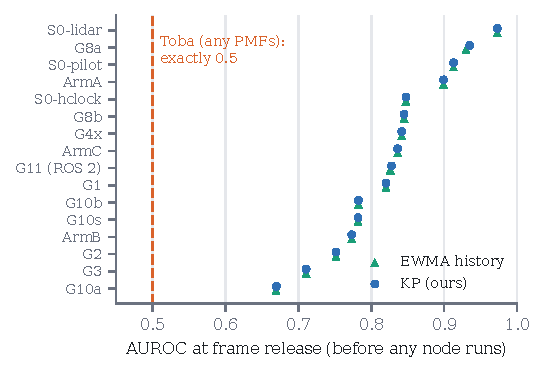
\includegraphics[width=0.62\textwidth]{figs/release_auroc.pdf}
\caption{Release AUROC per experimental case (57 hardware runs, 16 cases). The score of Toba et al. is constant at release
(Theorem~\ref{thm:blind}); any cross-frame state ranks frames.}
\label{fig:release}
\end{figure}

\begin{figure}[t]
\centering
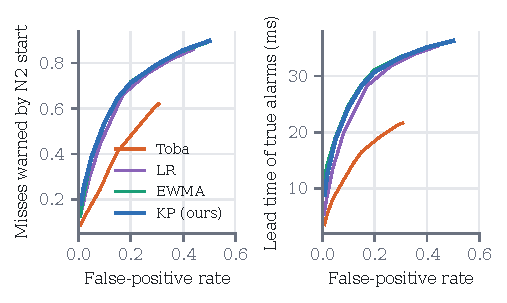
\includegraphics[width=0.62\textwidth]{figs/tradeoff.pdf}
\caption{The same alarm rule for every method with one threshold swept (mean of 57 runs). By the start of N2, history-based scores warn
about twice as many misses as plaxity, about twice as early.}
\label{fig:tradeoff}
\end{figure}

Fig.~\ref{fig:release} confirms Theorem~\ref{thm:blind}. Across 57 runs on two platforms, with synthetic and LiDAR workloads in Python,
C and ROS~2, the release AUROC of plaxity is exactly 0.5, and the history-based scores reach 0.64--0.97. The achieved AUROC tracks the
Gaussian prediction of Proposition~\ref{prop:limit} from the variance explained by the contention level (Spearman correlation
0.56--0.74), which explains the weak cases: where contention explains little of the latency, there is little to predict for any method.

\begin{table}[t]
\caption{Open-loop comparison (means). A: 57 runs; B: Raspberry Pi~5, six fresh runs (visual odometry / LiDAR)}
\label{tab:open}
\footnotesize
\begin{tabular}{@{}lccc@{}}
\toprule
& Toba et al.~\cite{toba2026} & KP / KPF & LR \\
\midrule
\multicolumn{4}{@{}l}{\emph{A. At the thresholds recommended in~\cite{toba2026}}}\\
FPR & 0.89 & 0.51 & 0.44 \\
Precision & 0.29 & 0.40 & 0.43 \\
\multicolumn{4}{@{}l}{\emph{A. At FPR = 10\%}}\\
Misses warned by the start of N2 & 0.25 & 0.54 & 0.45 \\
Lead time of true alarms (ms) & 11.6 & 24.4 & 20.2 \\
\multicolumn{4}{@{}l}{\emph{B. KPF and LR on all features}}\\
Actionable AUROC & 0.67 / 0.81 & 0.89 / 0.96 & 0.89 / 0.96 \\
FPR needed for the long-run guarantee & 0.35 / 0.20 & 0.12 / 0.09 & -- \\
\bottomrule
\end{tabular}
\end{table}

At the thresholds recommended in~\cite{toba2026}, plaxity raises an alarm on 89\% of the frames that meet the deadline; KP halves this
and is better in 53 of 57 runs (Table~\ref{tab:open}). With one threshold swept for all methods (Fig.~\ref{fig:tradeoff}), the precision
curves nearly coincide, but by the start of N2 KP warns 2.2 times more misses with 2.1 times the lead time. The actionable AUROC of KP
exceeds that of plaxity in 52 of 54 earlier runs and in 3 of 3 pre-registered ROS~2 runs (+0.14 to +0.27, block-bootstrap confidence
interval above zero). Theorem~\ref{thm:aci} held in all 1{,}140 checked cases, whereas a threshold fixed on calibration data drifted to
2--4 times its target under unseen contention. Meeting the same long-run guarantee required 1.5--3 times fewer false alarms with the
score of KP than with that of plaxity (106 of 114 cases).

These results do not show a better predictor. Logistic regression on the same features ranks frames as well as KPF or slightly better
(actionable AUROC 0.893 versus 0.888 on the UNO~Q), and the pre-registered test that KPF outranks it failed on both boards (2/6 and
3/6). A moving average of past latency captures most of the gain over plaxity. The remaining advantages of KPF are calibration under
unseen contention (expected calibration error 0.072 versus 0.128 for LR) and cost. In the open loop on the Pi~5, rule \Wu{} met
$(4,20)$ exactly (worst window 4.0, against 18.5 without a monitor and 7.3 with the burst guard alone) at an additional FPR of 0.012,
and it held for the scores of LR and of plaxity as well (36/36).

\subsection{Closed-Loop Evaluation: Latch-Up and Its Fix}\label{sec:eval-latch}

\begin{table}[t]
\caption{Closed loop on the Raspberry Pi~5 with the live ROS~2 LiDAR DAG, mean of three seeds (about 2{,}600 frames per policy). Last
column: worst number of unwarned misses in any 20 frames (for no action, misses that the passive monitor did not flag).}
\label{tab:latch}
\footnotesize
\begin{tabular}{@{}lcccc@{}}
\toprule
Policy & Missed & Degraded & Degraded in quiet periods & Worst unwarned per 20 \\
\midrule
No action & 36.7\% & 0\% & 0\% & 8 \\
Original monitor (\pol{kp}) & 9.4\% & 61.6\% & 30.0\% & 15.3 \\
Fixed monitor (\pol{kpm}) & 9.9\% & 43.8\% & \textbf{0.1\%} & 8 \\
Fixed monitor + \Wu{} (\pol{kpmwh}) & \textbf{8.7\%} & 43.1\% & 0\% & \textbf{4} \\
Toba et al.~\cite{toba2026} & 15.4\% & 48.4\% & 33.4\% & 10.7 \\
Random, same budget & 21.6\% & 43.5\% & 43.5\% & 16.7 \\
\bottomrule
\end{tabular}
\end{table}

Table~\ref{tab:latch} shows the pre-registered closed-loop experiment on the Pi~5 (8 of 9 rules passed). The mode-aware update reduced
degradation in quiet periods from 30\% to 0.1\% at the same miss rate, and rule \Wu{} held in every seed. Two results limit the claim.
The proposed method did not degrade fewer frames than plaxity (1/3 seeds), and frames degraded to level~1 were still late 10--16\% of the
time: halving the point cloud is a lighter mode, not a fallback. A later experiment on the UNO~Q isolated the fix from the burst guard:
the state update alone degraded 0--0.7\% of quiet frames, against 63--100\% for the original monitor. The pre-registered ratio rule for
``no latch'' still failed in two of three seeds, because its reference rate was exactly zero; it remains failed.

\subsection{Closed-Loop Evaluation: All Late Frames}\label{sec:eval-all}

\begin{figure}[t]
\centering
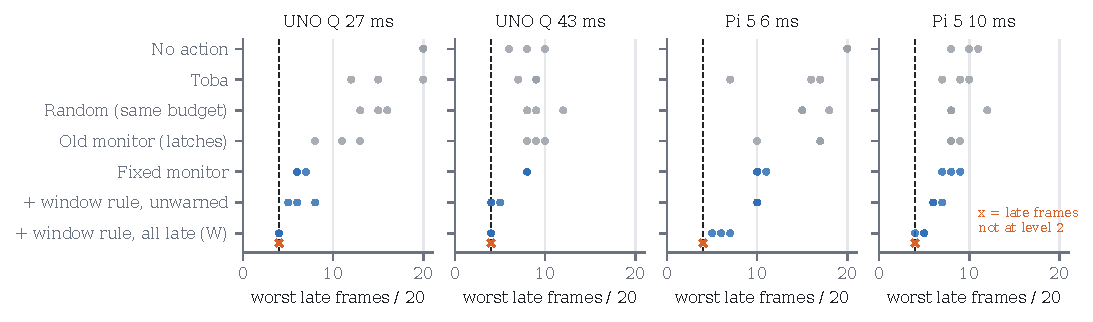
\includegraphics[width=\textwidth]{figs/closed_loop_windows.pdf}
\caption{Worst number of late frames in any 20-frame window per seed (dots), live ROS~2 closed loop. Dashed line: $m=4$. Crosses: late
frames not at level~2 under rule \Wl, which Theorem~\ref{thm:all} bounds by 4 without any timing assumption. UNO~Q at 27 and 43\,ms;
Pi~5 at 6 and 10\,ms; 2{,}000 frames per policy, seed and deadline.}
\label{fig:windows}
\end{figure}

Two pre-registered experiments ran all eight policies on fresh seeds at two deadlines per board (Fig.~\ref{fig:windows}).
\emph{Theorem~\ref{thm:all} held exactly in all 12 runs}: no window ever contained more than four late frames that were not at level~2.
On the UNO~Q, level~2 ran on 790 frames and none was late, so the plain form was met in all six runs: at most four late frames in every
window, under contention not seen in calibration, against 5--20 for the other policies at 27\,ms.

\emph{The Pi~5 at 6\,ms is a counterexample to the plain form, and it is reported as such.} Level~2 was late on 77 of 1{,}312 frames
(5.9\%), the worst window of all late frames reached 7, 5 and 6, and the pre-registered rule for the plain form failed (0/3). The
counterexample is to assumption A, not to the rule: every late frame beyond four in a window was a late level-2 frame, as
Theorem~\ref{thm:all} allows, and the worst window of late level-2 frames was 5, 1 and 5. Rule \Wl{} still had the smallest worst window
in every seed (7--20 for the other policies, with one tie) Its mean miss rate over the three seeds was 9.3\%, compared with
15.0\% for plaxity and 22.1\% for random degradation; this is a descriptive aggregate, not a claim that the proposed policy had the
lowest miss rate in every seed or a pre-registered result. At 10\,ms, two late level-2 frames in 243 were enough to exceed the plain
bound by one in two of three runs: a hard bound is broken by a single late fallback frame, however rare.

\subsection{Replication on Seven New Seeds}\label{sec:eval-repl}

To test whether the UNO~Q results depend on the three seeds above, the closed loop was repeated on seven new seeds (261--267) under an
addendum (Addendum S) frozen before any of its data existed. It reuses the eleven rules of the original experiment unchanged, the same
code and the same calibration procedure; the md5 sums of the rules, the analysis script and the board scripts were recorded at freezing.
One board reboot during seed 264 emptied an unflushed calibration file; that seed's calibration was rerun from the start, the lost
files are kept, and the phase script was changed only to flush files to disk. The calibration chose a 27\,ms heavy deadline on six seeds
and 26\,ms on one, and light deadlines of 42--44\,ms. Each of the 112 runs completed about 1{,}700--1{,}800 frames.

\emph{All rules about the guarantees passed.} Level-2 frames were on time in 14/14 runs (1{,}754 level-2 frames, none late), the exact
form of Theorem~\ref{thm:all} held in 14/14, the plain form held in 14/14 (worst window of all late frames exactly 4 in every
\pol{kpmd} run, against 11--20 for \pol{none}, \pol{toba} and \pol{random} at the heavy deadline), the long-run bound held in 42/42,
and the inline cost stayed below 200\,\textmu s at the 99th percentile in 14/14. Pooled over the ten UNO~Q seeds, Theorem~\ref{thm:all}
and Corollary~\ref{cor:A} held in 20/20 runs, and 0 of 2{,}544 level-2 frames were late (95\% upper bound 0.12\%).

\emph{Five comparative rules failed, and they remain failed.} The isolated update \pol{kpmn} did not latch in only 3/7 seeds under the
ratio rule (P5, needed 7/7). At the light deadline, \pol{kpm} missed fewer frames than no monitor in 4/7 seeds (P7a, needed 7/7) and no
more than random degradation at the same budget in 4/7 (P7b, needed 6/7); its mean miss rate over the ten seeds was 5.2\%, against
5.8\% without a monitor and 5.4\% for random degradation, so at light load the monitor does not reliably reduce misses. The spread of
degraded fractions was 0.31 for \pol{kpm} against 0.58 for plaxity, not below half (P8). The fallback rule \pol{kpmd} had no more late
frames than \pol{kpmwh} in 7/14 runs (P11, needed 12/14): the two are tied on total late frames, and the fallback buys the window bound on
all late frames, not fewer late frames. At the heavy deadline the mean miss rate over the ten seeds was 4.2--4.8\% for every policy with
the guarantee layer, against 33.3\% without a monitor, 16.4\% for random degradation and 18.0\% for plaxity (descriptive, not a rule).
The replication therefore confirms the guarantees and does not confirm the comparative advantages at light load.

\subsection{Validation of the Fallback Assumption}\label{sec:eval-fb}

\begin{figure}[t]
\centering
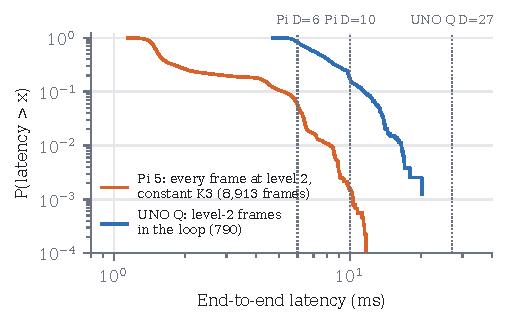
\includegraphics[width=0.62\textwidth]{figs/fallback_ccdf.pdf}
\caption{Latency tail of level-2 frames. Pi~5: stress runs with every frame at level~2 under constant contention with three
interferers (three seeds). UNO~Q: level-2 frames in the closed loop. The median frame on the Pi~5 takes 1.5\,ms, yet the tail reaches
12\,ms.}
\label{fig:fallback}
\end{figure}

Assumption A was tested directly with stress runs on the Pi~5, in which every scheduled release runs at level~2 under constant
contention with three interferers (Fig.~\ref{fig:fallback}). The experiment scheduled 4{,}000 releases for each of three seeds; the
analysis removes the releases that fall in a contention change and the first 20 remaining ones of each seed as warm-up, which leaves
8{,}913 retained frames. As predicted from a pilot, level~2 is not on time at 6\,ms: 2.3--10.2\% of the retained frames were late per
seed (3/3). At 10\,ms, 13 of the 8{,}913 retained frames were late (0.15\%; 95\% Clopper--Pearson~\cite{clopper1934} upper bound 0.23\%). The
tail is not caused by the amount of work: the median is 1.5\,ms, every level-2 divisor from 2 to 32 behaved alike in the pilot, and
pinning the interferers to other cores did not remove it. It is caused by operating-system scheduling under contention.

A follow-up experiment was pre-registered to test whether an unprivileged scheduling change, running the background load under
\texttt{SCHED\_IDLE}, makes level~2 on time at 6\,ms. The board became unreachable during the confirmatory runs and its data could not
be retrieved, so no result of that experiment is reported or used here.

Table~\ref{tab:ledger} states, for each guarantee, its premise and the evidence for that premise on each configuration. On the UNO~Q,
the evidence for A is 0 late frames out of 2{,}544 closed-loop level-2 frames over ten seeds, a 95\% upper bound of 0.12\% on the
per-frame late rate. A pre-registered stress test on this board (Addendum S, rule S12: at most 0.5\% late at 27\,ms) ran every frame at
level~2 under the heavy contention schedule for 4{,}000 releases on each of three seeds. With the same retention filter as on the Pi~5,
4 of 11{,}929 retained frames were late at 27\,ms (0.034\%; 95\% upper bound 0.077\%; rule passed), at most 3 in any window of 20, and
2 were late at 43\,ms; the median frame took 7.6--8.0\,ms and the worst 80\,ms. A is therefore \emph{supported} but not strictly true on
the UNO~Q: the fallback is late rarely, and a design should use Corollary~\ref{cor:r} with a small $r$ rather than Corollary~\ref{cor:A}. On the Pi~5 at 10\,ms the late rate is small and bounded but not zero,
so only Theorem~\ref{thm:all} and Corollary~\ref{cor:r} apply. On the Pi~5 at 6\,ms, A is false. The values of $r$ in
Table~\ref{tab:ledger} were measured on the same runs and therefore describe these runs; a design would need $r$ from separate
qualification runs. Late level-2 frames cluster (up to five in one window at a 5.9\% rate), so $r$ must be measured per window and
cannot be derived from the average rate under an independence assumption. The guarantees on \emph{unwarned} misses do not depend on A:
Theorem~\ref{thm:aci} held in all 36 policy runs of these two experiments, and the worst window of unwarned misses was exactly 4 in every
\pol{kpmwh} and \pol{kpmd} run on both boards.

\begin{table}[t]
\caption{Which window guarantee on late frames holds where (rule \Wl, $(m,K)=(4,20)$; UNO~Q: ten seeds at two deadlines, Pi~5: three seeds per deadline). ``Held'' and
``failed'' are observed outcomes; the premise is what a claim requires.}
\label{tab:ledger}
\footnotesize
\begin{tabular}{@{}p{0.27\textwidth}p{0.2\textwidth}ccc@{}}
\toprule
Guarantee & Premise & \makecell{UNO~Q\\27, 43\,ms} & \makecell{Pi~5\\10\,ms} & \makecell{Pi~5\\6\,ms} \\
\midrule
Theorem~\ref{thm:all}: late frames not at level 2 $\le m$ & none & held 20/20 & held 3/3 & held 3/3 \\
Corollary~\ref{cor:r}: late frames $\le m+r$ & at most $r$ late level-2 frames per window & $r=0$ & $r=1$ & $r=5$ \\
Corollary~\ref{cor:A}: late frames $\le m$ & A: level 2 never late & held 20/20 & \textbf{failed} 2/3 & \textbf{failed} 3/3 \\
\midrule
\multicolumn{2}{@{}l}{Late level-2 frames, closed loop} & 0 of 2{,}544 & 2 of 243 & 77 of 1{,}312 \\
\multicolumn{2}{@{}l}{Level-2 late rate, 95\% upper bound} & 0.12\% & 2.6\% & 7.1\% \\
\multicolumn{2}{@{}l}{Level-2 late, constant stress} & 0.034\% (27\,ms) & 0.15\% & 2.3--10.2\% \\
\multicolumn{2}{@{}l}{Status of assumption A} & supported (rare late) & false (rare) & false \\
\bottomrule
\end{tabular}
\end{table}

\subsection{Verification of the Theorems and the Implementation}\label{sec:eval-verify}

The proofs of Section~\ref{sec:method} are short, but a reviewer must be able to trust both the proofs and the claim that the deployed
code implements the rules they are about. Three independent checks were made.

\paragraph{Exhaustive state-space search} A first checker explores every reachable abstract state of rules \Wu{} and \Wl{} (38{,}900
states for $K\le7$, $m<K$ and lags up to 2, plus selected cases up to $K=10$). Its negative controls, a counter that ignores running
frames and a level~2 that can be late, are both caught.

\paragraph{Independent exhaustive enumeration} A second checker was written from scratch in C and shares no code with the first. It
enumerates every concrete sequence of predictor decisions, outcomes and completion delays of every frame up to a horizon $T$, for all
$K\le5$, $m<K$ and $L\le3$ ($T$ between 8 and 14), simulates the rules, and checks every window. In about 5.4 billion sequences it found
no violation of Theorems~\ref{thm:wu} and~\ref{thm:all} or of Proposition~\ref{prop:min}. It confirmed that a counter of known outcomes
only reaches exactly $\min(m+L-1,K)$ unwarned misses per window (Proposition~\ref{prop:need}(3)), so the lag effect is tight. It caught
an off-by-one variant of rule \Wu{} as a negative control. With integer arithmetic it enumerated every alarm and outcome sequence that
the threshold allows for $T\le14$, $L\le2$ and three initial thresholds, and found no violation of Theorem~\ref{thm:aci}. A third enumeration of the same kind checked Theorem~\ref{thm:cost} for all $K\le6$,
$m<K$ and $L\le3$ (about 15 billion sequences) and found no violation; for $L=1$ it found the largest $mF/U$ to be exactly $K-m$.

\paragraph{Implementation conformance} The logged closed-loop runs of Section~\ref{sec:eval-all} were replayed. For every release of
every \pol{kpmd} and \pol{kpmwh} run on both boards, the counter was recomputed from the logged completion times exactly as stated in
the rules, and the resulting decision was compared with the decision made by the deployed C++ code. All 48{,}000 release decisions
agreed, including UNO~Q runs in which frames took up to 289\,ms and therefore remained running across several releases. The same logs
satisfy Theorem~\ref{thm:cost} in all 12 \pol{kpmwh} runs: rule \Wu{} forced 2.3--12.5\% of the frames, against a worst-case bound of
$(K-1)U/m$ that was 2.6--7.7 times larger, because real misses do not arrive in the adversarial blocks of the worst case.

These checks are not formal proofs, and the enumeration covers small parameters only; they guard against errors in the reasoning and
in the implementation. The proofs themselves are the claim.

\subsection{Calculation Time and Downstream Value}\label{sec:eval-cost}

The inline monitor, including rule \Wl, takes 14--27\,$\mu$s per frame at the 99th percentile on the Pi~5 and 54--84\,$\mu$s on the
UNO~Q, less than 0.1\% of the period. Plaxity takes 3.6\,$\mu$s at the median on the UNO~Q. In a simulation driven by the recorded Pi~5
traces, an unstable plant under LQR control whose state estimate comes from the pipeline had 5--10 times lower control cost with KPF and
the guarantees than without a monitor, no crashes, and lower cost than with the score of plaxity (5 of 5 pre-registered rules). For this
plant, the certificate of Section~\ref{sec:all} gives a worst 20-frame block gain of 0.001--0.14 for all eight plant settings and six
budgets tried, while unbounded holds make the state grow 1.2--2.7 times per frame. The plant is simulated; the window bound that the
certificate needs was measured on hardware.

\subsection{Discussion and Limitations}\label{sec:eval-disc}

\paragraph{Choosing the window contract} The pair $(m,K)$ should be selected from the downstream controller's tolerance to consecutive
or clustered late outputs. The monitor enforces the selected contract; it does not determine whether a particular controller is stable
under that contract, so the certificate of Section~\ref{sec:all} must be evaluated for the intended plant and controller.
Corollary~\ref{cor:cost} gives the price side of the choice: the fraction of forced frames is at most $(K-1)\alpha/m$. Exploratory
UNO~Q runs, not part of the pre-registered rules, showed the expected trade-off: budgets much tighter than the long-run unwarned-miss
rate forced warnings on frames that the prediction layer considered safe.

\paragraph{Qualifying the fallback} Theorem~\ref{thm:all} is unconditional with respect to fallback timing. A designer should claim
the plain $(m,K)$ bound only when level~2 is established to be on time, for example by a WCET argument or a reservation. If occasional
level-2 misses remain, the designer must qualify a per-window budget $r$ independently and use Corollary~\ref{cor:r}. An average
fallback miss rate is not sufficient, because late level-2 frames cluster.

\paragraph{Choosing the predictor} Because the guarantee layer is score-agnostic, the predictor is an engineering trade-off among
false-alarm cost, calibration under unseen contention, implementation cost and available telemetry. A moving average of past latency
captured most of the gain over per-frame plaxity, and logistic regression ranked as well as or slightly better than KPF. The evidence
supports the value of cross-frame information, not a claim that the Kalman-based predictor is the best possible model.

\paragraph{Scope and threats to validity} The closed-loop evaluation uses one principal LiDAR DAG on two boards; repeated seeds on one
board are not independent hardware platforms. Visual odometry appears only in the open-loop replication. Toba's method was
re-implemented from the published equations because its original implementation was unavailable. The level-2 fallback has no WCET
proof. The downstream control experiment is driven by hardware traces but simulates the plant. The monitor was evaluated without
real-time priorities, CPU isolation or memory-bandwidth reservation; the effect of those mechanisms on the fallback tail is unmeasured.

\subsection{Summary of Claims, Premises and Status}\label{sec:eval-claims}

Table~\ref{tab:claims} lists every claim of the paper with its premise and status, including the claims that failed.

\begin{table}[t]
\caption{Claims, premises and status. ``Pre-registered'' gives the frozen rules passed out of the total.}
\label{tab:claims}
\footnotesize
\begin{tabular}{@{}p{0.43\textwidth}p{0.24\textwidth}p{0.25\textwidth}@{}}
\toprule
Claim & Premise & Status \\
\midrule
Plaxity cannot rank frames at release (Theorem~\ref{thm:blind}) & none & proven; observed in 57/57 runs \\
Cross-frame state ranks frames at release & contention present & AUROC 0.64--0.97 \\
The predictor outranks logistic regression & -- & \textbf{failed} (2/6, 3/6) \\
Long-run bound on unwarned misses (Theorem~\ref{thm:aci}) & none & proven; held in every run \\
$(m,K)$ on unwarned misses, minimal (Theorem~\ref{thm:wu}, Prop.~\ref{prop:min}) & none & proven; held in every run \\
All late frames, exact form (Theorem~\ref{thm:all}) & bookkeeping (verified) & proven; held 26/26 \\
All late frames, plain form (Corollary~\ref{cor:A}) & fallback never late & held 20/20 on UNO~Q; \textbf{failed} on Pi~5 (0/3 at 6\,ms, 1/3 at 10\,ms) \\
Fallback rarely late on the UNO~Q under stress & -- & 0.034\% late (S12 passed) \\
Replication on 7 new seeds, guarantee rules & -- & passed (P1--P3, P9, P10) \\
Replication, comparative rules & -- & \textbf{failed} (P5, P7a, P7b, P8, P11) \\
Fallback on time at 6\,ms on the Pi~5 & -- & \textbf{false} (pre-registered prediction) \\
Latch-up is fixed by the mode-aware update & -- & quiet-period degradation 30\% $\to$ 0.1\% \\
Fewer degraded frames than plaxity & -- & \textbf{failed} (1/3, twice) \\
Stability in the loop & window bound + plant & simulated plant only \\
\bottomrule
\end{tabular}
\end{table}

% =====================================================================================================================================
\section{Related Work}\label{sec:related}

This section provides an overview of research related to this paper. A comparative summary is presented in Table~\ref{tab:compare}.

Early detection of deadline misses for DAG tasks was introduced by Yano and Azumi~\cite{yano2023access}, who derived time constraints
for each job of mixed timer-driven and event-driven DAGs from the end-to-end deadline and WCETs. Toba and Azumi~\cite{toba2024} replaced
WCETs by probabilistic execution times, and Toba, Baruah and Azumi~\cite{toba2026} introduced workload-dependent probability thresholds.
These methods evaluate each job from its own elapsed time and assume independent execution times; the present paper adds cross-frame
state and a guarantee layer on top of their quantity. Pythia-MCS~\cite{jiang2020pythia} predicts overruns before they occur from I/O
behaviour to trigger mixed-criticality mode switches, but provides no window guarantee.

Probabilistic timing analysis convolves execution-time distributions to bound response times~\cite{bernat2002pwcet,davis2019survey}.
Markov and hidden-Markov models of execution times~\cite{frias2017,friebe2023} and correlation-tolerant
analyses~\cite{markovic2023cta,markovic2024caa} bound deadline-miss probabilities offline under dependence. They answer a design-time
question, whereas the proposed method decides online and uses the dependence caused by contention as information. Response-time analysis
of ROS~2 processing chains exists under reservation-based scheduling~\cite{casini2019ros2}; the platforms of this paper use none.
Memory-bandwidth regulation~\cite{yun2013memguard} reduces the contention that the proposed predictor exploits, and could also make a
fallback timely.

Weakly-hard constraints were formalized by Bernat, Burns and Llamos\'i~\cite{bernat2001weakly}. Bounded-miss
scheduling~\cite{bernat2001bms,hamdaoui1995} and weakly-hard monitoring~\cite{peeck2021,wu2020rv} are compared in detail in
Section~\ref{sec:position}. On the control side, deadline-miss-aware control~\cite{pazzaglia2019dmac} and stability analyses under
weakly-hard miss patterns~\cite{maggio2020,vreman2021} design or verify controllers for given miss patterns; the proposed method supplies
such a pattern on hardware, with its assumption measured. The Simplex architecture~\cite{sha2001simplex} is the template for the
fallback.

The long-run bound is the one-sided form of adaptive conformal inference~\cite{gibbs2021}. Validity when a model's outputs change its
own future inputs has been studied for design problems~\cite{fannjiang2022}; intervention latch-up is a concrete instance of this problem
in timing monitors.

% =====================================================================================================================================
\section{Conclusion}\label{sec:concl}

This paper presented a deadline miss early detection method for DAG tasks that remains correct when the system acts on its warnings.
It showed that per-frame plaxity cannot rank frames at release, and that a cross-frame contention state can. On top of any score, a
guarantee layer bounds the long-run rate of unwarned deadline misses and, with lag-correct counting and the fewest possible forced
warnings, the number of unwarned misses in every window. With a lighter fallback mode, it bounds all late frames in every window in an
exact form that states how the bound degrades when the fallback is late. The paper also identified and fixed intervention latch-up.
Pre-registered experiments on two embedded boards, an independent exhaustive check and an implementation conformance check confirmed
the theorems exactly. They also showed that the plain bound on late frames holds only where the fallback is on time: it was met on the
UNO~Q, including a replication on seven new seeds, and failed on the Raspberry Pi~5 at 6\,ms, where the exact form is the guarantee to
use. The replication did not confirm the comparative advantages: at light load the monitor did not reliably reduce misses, and the
fallback did not reduce the total number of late frames.

Future work will focus on establishing the timeliness of the fallback rather than measuring it: running the fallback under a
reservation~\cite{casini2019ros2} or with memory-bandwidth regulation~\cite{yun2013memguard} on a platform where such mechanisms are
available, and deriving the budget $r$ of Corollary~\ref{cor:r} from qualification runs. Future work will also extend the evaluation to
multi-rate DAGs with timer-driven and event-driven nodes as in~\cite{yano2023access,toba2026}, and to a physical control loop instead of a
simulated plant.

\begin{acks}
Withheld for double-blind review.
\end{acks}

\bibliographystyle{ACM-Reference-Format}
\bibliography{refs}

\end{document}
